% \vspace{-0.4\baselineskip}
\section{Approach}
% \vspace{-0.4\baselineskip}
\label{sec:approach}

\begin{figure*}[ht!]
\centering
% \vspace{-0.5\baselineskip}
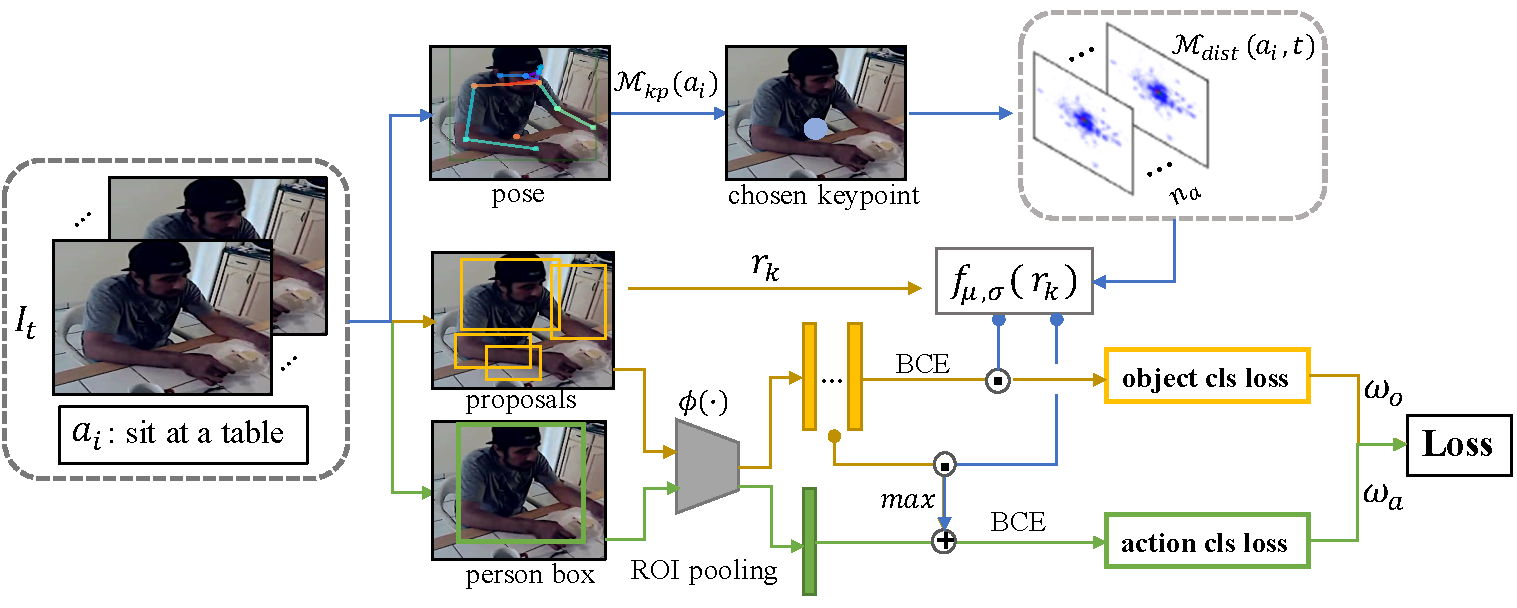
\includegraphics[width=0.8\textwidth]{figures/pipeline.pdf}
% \caption{Visual comparison of depth and normal results between \protect\cite{zhou2017unsupervised} and ours. As the original depth ground truth map comes from sparse laser measurement, the interpolated depth map is shown for better visualization. As can be seen from the depth estimation, our results preserve the small/thin structures which have similar color to other foregrounds (green circles). From the normal comparison, our results predict the road normal direction better and have no artifact. The edges in normal map are also preserved better in our results (yello circles).}
\caption{The object appearance is learned with a weakly supervised method by leveraging the three regularizations.}
% \vspace{-0.8\baselineskip}
\label{fig:pipeline}
\end{figure*}
% As discussed in \secref{sec:intro}, one major problem is that both~\cite{zhou2017unsupervised} and~\cite{yang2018aaai} have the regularization performed \wrt image gradient, which blocks nonlocal smoothness due to many false positives such as boundaries of shadows. 
In this section, we introduce the framework and different regularizations we have applied in detail.
\subsection{Overview}
% In this section, we introduce the regularizaitons we apply to learn the object representation via supervision from action labels. To better show our analysis, the information that can be leveraged are listed in different axis in \figref{fig:analysis}. Basically, we propose to explore three constraints to help learning object appearance. The first one includes the appearance consistency of objects in the same action class (blue box in \figref{fig:analysis}). The other constrain comes from the motion consistency in the same action class. The motion of ``drinking water from cup/bottle'', including both subject and object motion, is similar across videos. Last but not least, the object appears similarly in videos of different action labels but involving same object category. In the actions ``holding vacuum'' and ``fixing vacuumm'' (green box in \figref{fig:analysis}), object appearances are consistent.
As stated before, we propose to leverage appearance and motion consistency in the interaction between person and objects. The motion consistency is modeled by modeling the correlation between spatial location change with time, between person and interacted objects. Practically, such correlation is modeled between the person joint and object locations. The person joints (keypoints) are firstly estimated with off-the-shelf method and a dominant keypoint is chosen automatically by the pipeline. Attention maps around the chosen keypoint are estimated to model the probability of object locations. Class agnostic proposals are generated in a bottom-up way and weighted with the attention maps. The weighted proposals are then fed into action classification and object classification modules respectively. The action classification module takes object proposals and person detection bounding box as input and outputs action classification scores. Binary cross-entropy loss is calculated as supervision. Object classification module takes proposals as input and logistic losses are calculated for each object class as supervision. The weighted sum of the two losses is the final loss for the whole framework. 

\subsection{Framework}

Formally, for a given training video, the provided annotations include a set of action labels $\scr{L}$ = {$l_1,...,l_n$}. Each action label consists of an action class $a_i$ and corresponds to a clip in the video. The action class $a_i$ belongs to a predefined action set $a_i \in \scr{A}$, which is of size $n_{a}$: $||\scr{A}||=n_{a}$. All actions are interactive and there is one object class involved in each action $a_i\rightarrow o_{m(i)}, o_{m(i)}\in \scr{O}$. For example, object class \textit{cup} appears in the action \textit{holding a cup}. $m$ is a mapping from action class to object class. There are $n_{o}$ object classes: $||\scr{O}||=n_{o}$ in total. During training, clip-level action class $a_i$ and corresponding object class $o_{m(i)}$ are used as supervision signal.

\figref{fig:pipeline} illustrates an overview of our approach. $\scr{K}$ frames are uniformly sampled from each clip and are processed with a person detector and pose estimation network to generate person bounding box $P_t$ and human key point detection results $K_t$ for each frame $f_t$. We focus on the person with highest detection confidence. The number of keypoints is $n_{kp}=||K_t||$. Class-agnostic proposals $R_t$ are generated with bottom-up methods as candidate bounding boxes. The number of proposals is fixed to be $n_R=||R_t||$. To model the correlation between action and object motion, a keypoint is automatically chosen for a given action class. A spatial distribution is estimated to model the probability of object's location on each sampled frame. Appearance features ($\phi(R_t), \phi(P_t)$) are extracted from proposals $R_t$ and person bounding box $P_t$. The proposal features are fed into the object classification module along with the object location probability. The person feature is fused with proposal features and are fed into the action classification module. The weighted sum of two classification losses serve as our supervision of the pipeline.

% The action class labels are leveraged in the action classification stream. The person bounding box is processed with the same convolutional network to extract the person visual features $\phi(P_t)$. Similar to the multiple instance learning idea in \cite{gkioxari2015contextual}, the person region feaures are fused with the proposal region features $\phi(R_t)$ and then fed into the action classification module. As shown in \figref{fig:task_definition}, there may be overlap between different annotated clips, and thus it poses the action classification as a multi-label problem. The binary cross-entropy loss is used as action classification supervision. The object and action classification losses are weighted summed as the final loss term.

\subsection{Attention modeling}
We introduce the attention module for modeling the correlation between person and object motion. In practice, the attention is modeled with two steps: (1) attention on human keypoints and (2) attention for object loactions with regard to the keypoint. The modeling of attention is based on our observations that for a given action, there is often one human joint that is significantly involved. And there is tight spatial location correlation between the keypoint and object. For example, in the action \textit{drink from a cup}, the locations of \textit{hand} (joint) and \textit{cup} (object) are relatively fixed. In the action \textit{kicking a ball}, the relative motion between \textit{foot} and \textit{ball} is predictable and can be modeled.

Formally, the keypoint attention is modeled with a mapping $\hua{M}_{kp}$ from action class $a_i$ to chosen keypoint. 
\begin{align}
K_t^{a_i} = \hua{M}_{kp}(a_i)
\end{align}
The keypoint of interest is only dependent on the action class.
% For each action class, there will be a vector weighting for different keypoints. The top weighted keypoint is chosen as the point of interest for each action class. 
Given an action class $a_i$ and time step $t$, the attention for object location \wrt keypoint is modeled with a learned distribution in 2D space: $\scr{N}(\ve{\mu}_i^t, \ve{\sigma}_i^t)~~\ve{\mu}_i^t\in \mathbbm{R}^2, \ve{\sigma}_i^t\in \mathbbm{R}^{(2\times2)}$. $\ve{\mu}_i^t$ represent the normalized mean location of distribution center \wrt the chosen keypoint. The density function of such distribution is used to calculate the probability of different locations. Specifically, the probability of object being at the location of some proposal $r_k\in R_t$ is 
\begin{align}
w_k^{a_i}=f_{(\mu_i^t, \sigma_i^t)}(L(r_k)-K_t^{a_i})
\end{align}
$L(r_k)$ is the center of the proposal. The object location attention is modeled dependent on both action class and time step, to model both the relative spatial location and motion correlation. 

\subsection{Object classification}
The features are extracted from each proposal region $\phi(r_k), r_k \in R_t$ (superscript $t$ is omitted in $r_k^t$ for simpler symbol). An $n_o$-dimensional classification score is generated by applying object classification fully connected (\textit{fc}) layer on appearance features: $s_o(r_k) = fc_o(\phi(r_k))$ for each proposal. Unlike only leveraging image-level object labels for classification \cite{bilen2016weakly,kantorov2016contextlocnet}, the attention probability guided the approximate locations of objects and thus is leveraged in our object classification module. Formally, for any frame $I_t$ in a clip with action class $a_i$, the distribution probability at all proposals' locations can be calculated. The object classification loss incorporates the proposals features and distribution probabilities:
\begin{align}
\label{eqn:obj_cls_loss}
&\hua{L}_{obj} (I_t) = -\frac{1}{n_R\cdot n_o}\sum_{k}^{n_R}\sum_{j}^{n_o} f(L(r_k)-K_t^{a_i}) \cdot \nonumber \\
&~~~~~~~~~~~~~~~~w_k^{a_i}log(P(o_j|r_k))+(1-w_k^{a_i})log(1-P(o_j|r_k)), \nonumber\\
&P(o_j|r_k) = \frac{exp(s_o(r_k)_j}{\sum_{j}^{n_o}exp(s_o(r_k)_j)}
\end{align}

\subsection{Action classification}
For the task of action recognition, especially for interactive actions as in our task, both the person and the object appearances are vital cues. As indicated in \cite{gkioxari2015contextual}, the spatial location of the most informative object, which is often the one that the person interacted with, can be mined from action recognition task. We incorporate similar idea into our pipeline by fusing the proposal region and person region features. Formally, on given frame $I_t$ in the clip with action label $a_i$, the appearance features of both person region $P_t$ and proposal regions $R_t$ are extracted and then linearly transformed into an $n_a$-dimensional score: $s_a^o(r_k) = fc_a^o(\phi(r_k))$ and $s_a^a(P_t) = fc_a^a(\phi(P_t))$ correspond to action classification scores from proposal regions and person regions respectively. The proposal scores and person scores are weighted combined using distribution probabilities. And the cross entropy loss is calculted as the action classification loss. The formulation is shown in \equref{eqn:act_cls_loss}.

\begin{align}
\label{eqn:act_cls_loss}
&\hua{L}_{act} (I_t) = -\frac{1}{n_R\cdot}\sum_{k}^{n_R} log(P(\alpha=a_{i_t}|r_k)), \nonumber\\
&P(a_i|r_k) = \frac{exp(s_a^a(r_k)_{\alpha}+s_a^o(r_k)_i*w_k^{a_i})}{\sum_{i}^{n_a}exp(s_a^a(r_k)_{i}+s_a^o(r_k)_{i}*w_k^{a_i})}
\end{align}

\subsection{Loss terms}
The final loss is a weighted sum of the above loss terms. The hyperparameters $w_o$ and $w_a$ are weights to trade off the relative importance of object classification and action classification in the pipeline.
\begin{align}
\label{eqn:final_loss_term}
\hua{L}(\scr{F}, \scr{A}, \scr{O}) = \frac{1}{||\scr{F}||}(w_o\hua{L}_{obj}+w_a\hua{L}_{act})
\end{align}

